\begin{frame}{}

  \setlength{\parindent}{0pt}

  \vspace{-0.2cm}
  %% \begin{tabular}{ | p{0.44\textwidth}  | p{0.001\textwidth} | p{0.44\textwidth} |}
      \begin{tabular}{  p{0.43\textwidth}   p{0.02\textwidth}  p{0.43\textwidth} }

\onslide<1->{\only<1-7>{
    \begin{center}
      \mbox{\myul{\textit{\textbf{Standard random network model}}}}
    \end{center}}}       

    &&
    \onslide<4->{
    \begin{center}
      \mbox{\myul{\textit{\textbf{Varying connection probabilities}}}}
    \end{center}}

    \\
%
        \onslide<1->{\only<1-7>{%
    \vspace{-0.8cm}\begin{center}%
      \includegraphics[width=0.69\linewidth]{%
        figures/tikz_line.pdf} %
    \end{center}}%
        \only<8-10>{\begin{figure}%
            \centering\vspace{-0.6cm}
          \includegraphics[width=0.2\textwidth]{%
          /home/fh/two_point_network/two_point_network.pdf} %
      \end{figure}}
        }

    %             \onslide<1->{
    %     \begin{center}%
    %   \includegraphics[width=0.69\linewidth]{%
    %     figures/tikz_line.pdf} %
    % \end{center}}%
    %     \only<8-9>{\begin{figure}%
    %       \centering%
    %       \includegraphics[width=0.2\textwidth]{%
    %       /home/fh/two_point_network/two_point_network.pdf} %
    %     \end{figure}}}

    &&

       \onslide<4->{
    \begin{center}\vspace{-0.71cm}
      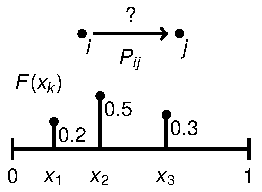
\includegraphics[width=0.69\linewidth]{%
        figures/tikz_line_right.pdf} % 
    \end{center}%\vspace{1cm}
       }
    \\
    \onslide<1->{   \vspace{-0.27cm} 
    Probability of connection a \myul{constant} $P_{ij}$,
    %\vspace{0.05cm}

    \begin{align*}
      P_{ij} = c
    \end{align*}
}
    &&

       \onslide<5->{\vspace{-0.27cm}
    Probability of connection a \myul{random variable} $P_{ij}$,
    \vspace{0.01cm}
    
    \begin{align*}
      \mathbf{Prob}(P_{ij}=x_k) = F(x_k)
    \end{align*}}	

    \\

        \onslide<2->{\vspace{-0.88cm}
    \textbf{Overall connection probability}
    \vspace{0.12cm}
    
    \begin{align*}
      \mu = P_{ij} = c
    \end{align*}}


    &&
    \onslide<6->{\vspace{-0.88cm}
    \textbf{Overall connection probability}
    \vspace{-0.08cm}
    
    \begin{align*}
      \mu = \sum_{k=1}^m F(x_k) x_k
    \end{align*}}
    
    \\
    \onslide<3->{\vspace{-0.8cm}
    \textbf{Bidirectional connection}
    \vspace{0.12cm}
    
    \begin{align*}
      P_{\text{bidir}} = P_{ij} P_{ji} = c^2
    \end{align*}	}

    &&
    \onslide<7->{\vspace{-0.8cm}
    \textbf{Bidirectional connection}
    \vspace{-0.08cm}

       \only<7-8>{\vspace{0.18cm}
    \begin{align*}
      P_{\text{bidir}} = \text{?} %\label{eq:TT}
    \end{align*}}
       \only<9-10>{
    \begin{align*}
      P_{\text{bidir}} = \sum_{k=1}^m \sum_{l=1}^m F(x_k) x_k \only<9>{F(x_l | x_k)}\only<10>{\myul[red]{F(x_l | x_k)}} x_l %\label{eq:TT}
    \end{align*}}}
    
  \end{tabular}

  
  % \source{\cite{Hoffmann2017}}
  
\end{frame}




\begin{frame}{}

    % 
    \begin{columns}
      % 
      \begin{column}{.5\textwidth}
        \minipage[c][0.85\textheight][s]{\columnwidth}

        \onslide<2->
        \begin{align*}
          P_{\text{bidir}} &= \sum_{k=1}^m \sum_{l=1}^m F(x_k) x_k F(x_l | x_k) x_l \\ &= \sum_{k=1}^m F(x_k) x_k^2 .
\end{align*}


\onslide<3->
\textit{Relative overrepresentation} $\varrho$ is the fraction

\begin{align*}
  \varrho = \frac{P_{\text{bidir}}}{\mu^2} = \frac{\sum_{k=1}^m F(x_k) x_k^2 }{\left(\sum_{k=1}^m F(x_k) x_k\right)^2}.
\end{align*}

\onslide<4->
By Jensen's inequality,

\begin{align*}
  \left(\sum_{k=1}^m F(x_k) x_k\right)^2 \leq \sum_{k=1}^m F(x_k) x_k^2  \quad \text{and thus} \quad \varrho \geq 1.
\end{align*}	

        
        \endminipage      
      \end{column}
      % 
      \begin{column}{.5\textwidth}
        \onslide<1->
        \minipage[c][0.85\textheight][s]{\columnwidth}

        \onslide<1->\begin{align*}
  F(x_l | x_k) = \begin{cases} 1 & \text{if $l = k$} \\ 0 & \text{otherwise.} \end{cases}
        \end{align*}


        
        \begin{figure}
          \centering
          \includegraphics[width=0.85\textwidth]{%
          /home/fh/sci/rsc/nrnd_pairs/pub/arxiv_16/figures/two_point_network/two_point_network.pdf} %
      \end{figure}

      \vspace{1.25cm}
        
        \endminipage
        
        
      \end{column}
    \end{columns}
    \onslide<1>\source{\normalsize \cite{Hoffmann2017}}
    
  \end{frame}

%   \begin{frame}
  
% \begin{align*}
%   F(x_l | x_k) = \begin{cases} 1 & \text{if $l = k$} \\ 0 & \text{otherwise.} \end{cases}
% \end{align*}
% Then


% \vspace{0.4cm}

% \textit{Relative overrepresentation} $\varrho$ is the fraction

% \begin{align*}
%   \varrho = \frac{P_{\text{bidir}}}{\mu^2} = \frac{\sum_{k=1}^m F(x_k) x_k^2 }{\left(\sum_{k=1}^m F(x_k) x_k\right)^2}.
% \end{align*}
% By Jensen's inequality,

% \begin{align*}
%   \left(\sum_{k=1}^m F(x_k) x_k\right)^2 \leq \sum_{k=1}^m F(x_k) x_k^2  \quad \text{and thus} \quad \varrho \geq 1.
% \end{align*}	
% %% If and only if $m > 1$, that is when the probability distribution of connection probabilities is non-degenerate, strict inequality in (2) holds.  

% \source{\normalsize \cite{Hoffmann2017}}
% \end{frame}


  \begin{frame}{}

    \begin{figure}
    \centering
    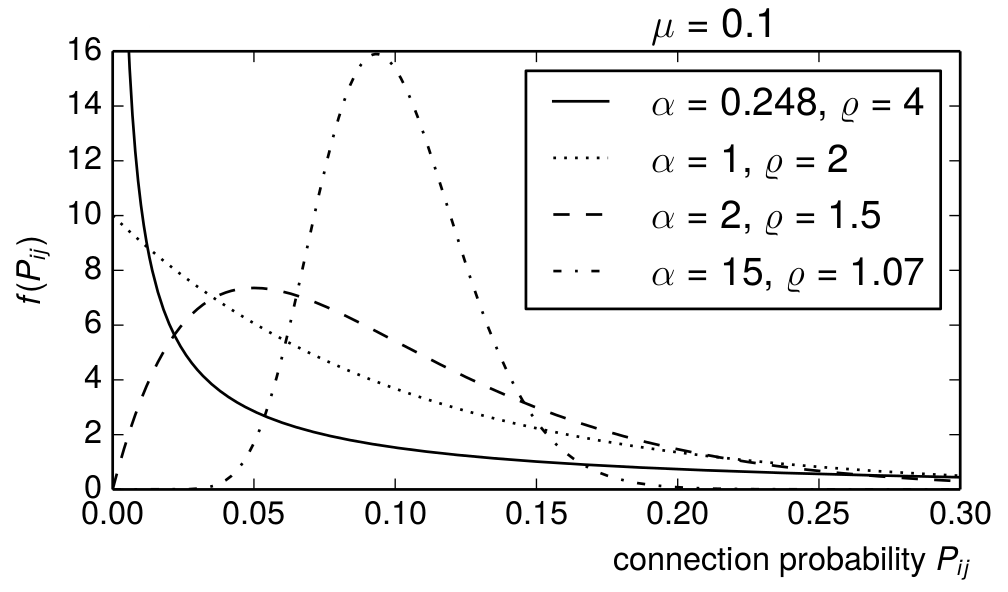
\includegraphics[width=0.8\textwidth]{%
      figures/nrnd_gamma.png} %
  \end{figure}

  \vspace{0.2cm}

  \begin{itemize}[leftmargin=1.3cm]
    \large
    \itemsep9pt
  \item[--]<2-> multiple neuron properties together can cause strong overrepresentation
  \item[--]<3> example: higher connection probability in functionally
\\    related cells \parencite{Lee2016a}

       
  \end{itemize}

  \vspace{0.4cm}
  
  

  \source{\normalsize \cite{Hoffmann2017}}
  
\end{frame}




